% Created 2017-03-28 Ter 13:43
% Intended LaTeX compiler: pdflatex
\documentclass{report}
               \pagestyle{fancy}
\usepackage[utf8]{inputenc}
\usepackage[T1]{fontenc}
\usepackage{graphicx}
\usepackage{grffile}
\usepackage{longtable}
\usepackage{wrapfig}
\usepackage{rotating}
\usepackage[normalem]{ulem}
\usepackage{amsmath}
\usepackage{textcomp}
\usepackage{amssymb}
\usepackage{capt-of}
\usepackage{hyperref}
\usepackage{paralist}
\usepackage{tcolorbox}
\usepackage[table]{xcolor}
\usepackage{lipsum}
\usepackage{caption}
\usepackage{tabu}
\usepackage[subpreambles=true]{standalone}
\usepackage{import}
\usepackage{setspace}
\usepackage{graphics}
\usepackage[linktocpage=true]{hyperref}
\usepackage{tocloft}
\usepackage{minitoc}
\usepackage[portuguese, english]{babel}
\usepackage[utf8]{inputenc}
\usepackage{subfig}
\date{}
\title{}
\hypersetup{
 pdfauthor={user},
 pdftitle={},
 pdfkeywords={},
 pdfsubject={},
 pdfcreator={Emacs 25.1.1 (Org mode 9.0.5)},
 pdflang={English}}
\begin{document}

\thispagestyle{firstpagestyle}
\IssueTitle{Time for Market Discipline}
\NewsAuthor{Joao Mauricio Rosal, \small\it Chief Economist, PhD}
\NewsEmail{joao.rosal@bgcpartners.com}
\JournalIssue
    \begin{tcolorbox}[colbak=red!5!white, colframe=red!0!white]
      \NewsItem{Time for Market Discipline}
      \begin{compactitem}
      \item \textit{We understand the balance of risks have somewhat tilted to the downside as the odds of a muddling through type of social security reform have increased.}
      \item \textit{This implies a two-fold path going forward: either a) market discipline forces the political class to embrace a meaningful reform (our base-case),
                    or b) political forbearance leads to a soft version, with negative impact on local assets.}
      \item \textit{The odds of a volatility free path towards a significant reform seems very low at moment.}
      \end{compactitem}
    \end{tcolorbox}
\vspace{-0.5cm}


\section{Market Discipline}
\label{sec:orgee9a00d}
\begin{compactitem}[$\diamond$]
\item \textbf{Balance of risks have tilted down}. The latest flow of news have
confirmed the difficulties of Mr. Temer to approve his social
security reform as is. While some type of compromising has been
expected from the outset, we believe the latest announcement that
Mr.Temer may leave State civil servants out of the reform has opened
a Pandora box, making more difficult to predict what is going to
come out of it. As matter of fact, the government itself has
understood the complexity of the move, and is - reportedly -
attempting to take a u-turn on the issue.

\item \textbf{The Genie is out}. Simply put, once one makes a
compromising to a specific class of entrenched interests, the
incentives are such that other organized classes should soon start
to lobby for the same type of favoritism. In addition, there is also
the interest of less organized citizens, such as those living off
social benefits, who are held pretty close to the heart of
politicians in Brasilia. Therefore, if one sums all that up, the
budget of acceptable concessions may run the risk of falling short
of the mounting pressures, a question mark we will need get
accustomed to in the next few months.

\item \textbf{Any counteracting pressure?} In light of the aforementioned, the
easy path towards a reform that comprises a) an increases the
minimum retirement age to 65 for both genders; b) the end of the
retirement linked to the number of years contributing to the system;
and c) encompasses rural, urban, private and public workers alike,
looks very slim. In fact, if we are to witness any satisfactory
compromising, counteracting forces against the softening pressures
are of paramount importance, and in this respect, the market looks
like the only candidate that may take up this role. In other words,
reform without volatility looks close to a contraction at moment.

\item \textbf{The Room for Discipline}. In fact, as in the exhibit
\ref{fig:spreads}, Brazilian sovereign spreads have been standing
about 90bps above Mexico's year-to-date, a country holding a
sovereign credit rating about 4 notches above Brazil's. No doubt, it
entails a rather benign vision towards the Brazil's fiscal outlook,
in particular, with respect to the country social security system.
Hence, should this perception changes significantly, there is plenty
of room for things to turn sour. In fact, the recent moves
concerning the social security reform have not been shrugged off by
the market, and the volatility of Brazilian assets have clearly take
off from the US' benchmark (\ref{fig:vol}).
\end{compactitem}

\begin{figure}[h]\centering
\subfloat[]{\label{fig:spreads}
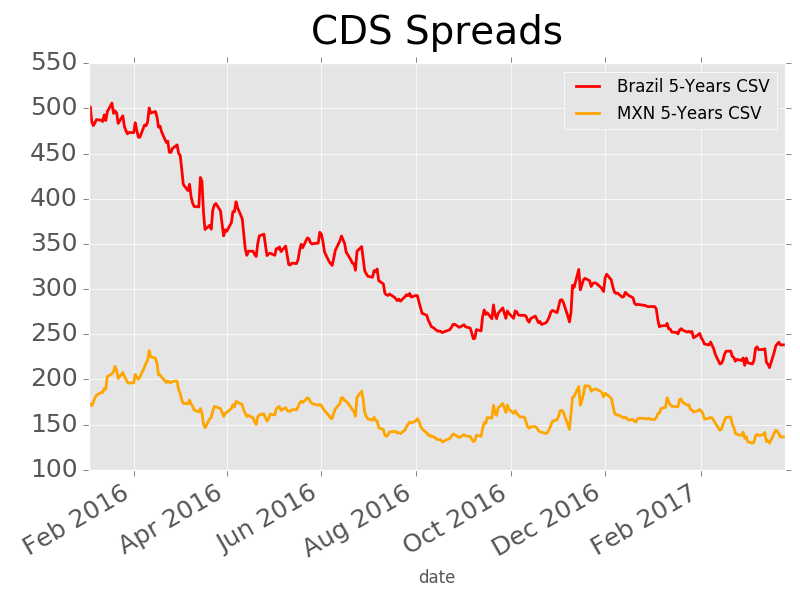
\includegraphics[width=7.5cm]{./images/csv.png}
}
\subfloat[]{\label{fig:vol}
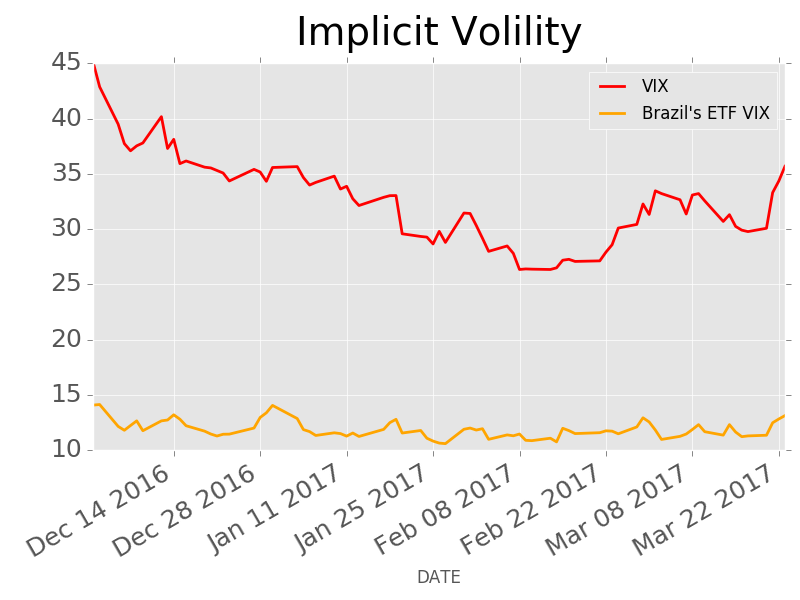
\includegraphics[width=7.5cm]{./images/vix.png}
}
\end{figure}

\begin{itemize}
\item \textbf{Forecasts unchanged for now}. Risk balances aside, we stick to the
vision that the Selic rate should reach 8.00\% by year-end, including
a couple 100bps cuts in the next two COPOM meetings. Our thesis
relies on inflation drivers as opposed to any hypothesis concerning
structural rate debate, and provided no major dislocation of the
market occurs, this story should remain intact.
\end{itemize}

\newpage


\section{Forecasts}
\label{sec:orgde650d2}

\rowcolors{2}{grey!15}{white}
\begin{center}
\begin{tabular}{lrrr}
\hline
\textbf{Variable} & \textbf{2016} & \textbf{2017E} & \textbf{2018E}\\
\hline
\hline
GDP (yoy \%) & -3.5 & 0.3 & 2.5\\
Selic Rate (\%) & 13.25 & 8.00 & 7.5\\
Fx Rate (BRL per USD) & 3.20 & 3.25 & 3.30\\
CPI (yoy \%) & 6.3 & 4.0 & 4.4\\
Gross Debt to GDP (\%) & 73.0 & 77.2 & 83.2\\
Primary Surplus (\% GDP) & -2.1 & -2.0 & -1.0\\
Trade Balance (\% GDP) & 2.0 & 1.5 & 1.5\\
Current Account (\%GDP) & -1.2 & -1.5 & -2.0\\
Foreign Reserves (xUSD Gross Liabilities) & 1.1 & 1.1 & 1.1\\
\hline
\end{tabular}
\end{center}
\newpage


\section{Disclaimer}
\label{sec:org718fe4d}
\url{http://www.bgcpartners.com} \\
\textbf{CONFIDENTIAL:} This document has been sent to you by one of
the BGC entities (collectively BGC) Please see important legal
information and disclaimer relating to this mail at the following
links: \url{http://www.bgcpartners.com/disclaimers/}

Please see for BGC Disclosures. The link contains company and FCA
registration numbers. This e-mail, including its contents and
attachments, if any, are confidential. If you are not the named
recipient please notify the sender and immediately delete it. You may
not disseminate, distribute, or forward this e-mail message or
disclose its contents to anybody else. Copyright and any other
intellectual property rights in its contents are the sole property of
BGC and its affiliates. E-mail transmission cannot be guaranteed to be
secure or error-free.  The sender therefore does not accept liability
for any errors or omissions in the contents of this message which
arise as a result of e-mail transmission.  If verification is required
please request a hard-copy version. Although we routinely screen for
viruses, addressees should check this e-mail and any attachments for
viruses. We make no representation or warranty as to the absence of
viruses in this e-mail or any attachments. Please note that to ensure
regulatory compliance and for the protection of our customers and
business, we may monitor and read e-mails sent to and from our
server(s).  The registered offices of the BGC entities are at 1
Churchill Place, London, E14 5RD.  For any issues arising from this
email please reply to the sender.  The FCA register appears at
\url{http://www.FCA.org.uk/register/}.  The FCA regulates the financial
services industry in the United Kingdom and is located at 25 The North
Colonnade, Canary Wharf, London, E14 5HS.  BGC Financial LP CFTC Rule
1.55(K) Firm Specific Disclosure Statement
\end{document}
